\documentclass[tikz]{standalone}
\usepackage{fourier}
\usepackage{tikz}

\begin{document}
	%:-+-+-+-+- Engendré par : http://math.et.info.free.fr/TikZ/TableauxVariations/
	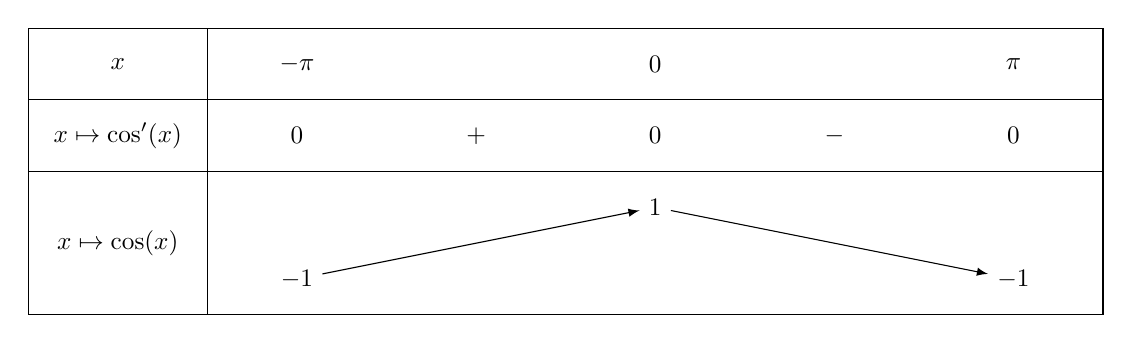
\begin{tikzpicture}[thick,scale=0.91, every node/.style={scale=0.91}]
		% Styles
		\tikzstyle{cadre}=[thin]
		\tikzstyle{fleche}=[->,>=latex,thin]
		\tikzstyle{nondefini}=[lightgray]
		% Dimensions Modifiables
		\def\Lrg{2.5}
		\def\HtX{1}
		\def\HtY{0.5}
		% Dimensions Calculées
		\def\lignex{-0.5*\HtX}
		\def\lignef{-1.5*\HtX}
		\def\separateur{-0.5*\Lrg}
		% Largeur du tableau
		\def\gauche{-1.5*\Lrg}
		\def\droite{4.5*\Lrg}
		% Hauteur du tableau
		\def\haut{0.5*\HtX}
		\def\bas{-2.5*\HtX-2*\HtY}
		\fill [white] (\gauche, \haut) rectangle (\droite,\bas);
		% Ligne de l'abscisse : x
		\node at (-1*\Lrg,0) {$x$};
		\node at (0*\Lrg,0) {$-\pi$};
		\node at (2*\Lrg,0) {$0$};
		\node at (4*\Lrg,0) {$\pi$};
		% Ligne de la dérivée : f'(x)
		\node at (-1*\Lrg,-1*\HtX) {$x \mapsto \cos'(x)$};
		\node at (0*\Lrg,-1*\HtX) {$0$};
		\node at (1*\Lrg,-1*\HtX) {$+$};
		\node at (2*\Lrg,-1*\HtX) {$0$};
		\node at (3*\Lrg,-1*\HtX) {$-$};
		\node at (4*\Lrg,-1*\HtX) {$0$};
		% Ligne de la fonction : f(x)
		\node  at (-1*\Lrg,{-2*\HtX+(-1)*\HtY}) {$x \mapsto \cos(x)$};
		\node (f1) at (0*\Lrg,{-2*\HtX+(-2)*\HtY}) {$-1$};
		\node (f2) at (2*\Lrg,{-2*\HtX+(0)*\HtY}) {$1$};
		\node (f3) at (4*\Lrg,{-2*\HtX+(-2)*\HtY}) {$-1$};
		% Flèches
		\draw[fleche] (f1) -- (f2);
		\draw[fleche] (f2) -- (f3);
		% Encadrement
		\draw[cadre] (\separateur,\haut) -- (\separateur,\bas);
		\draw[cadre] (\gauche,\haut) rectangle  (\droite,\bas);
		\draw[cadre] (\gauche,\lignex) -- (\droite,\lignex);
		\draw[cadre] (\gauche,\lignef) -- (\droite,\lignef);
	\end{tikzpicture}
	%:-+-+-+-+- Fin
\end{document}